\documentclass{tufte-handout}

%\geometry{showframe}% for debugging purposes -- displays the margins

\usepackage{amsmath}

% Set up the images/graphics package
\usepackage{graphicx}
\setkeys{Gin}{width=\linewidth,totalheight=\textheight,keepaspectratio}
\graphicspath{{graphics/}}

\title{ArmoredSoftware: Trust in the Cloud}
\author{Perry Alexander, The University of Kansas}

% The following package makes prettier tables.  We're all about the bling!
\usepackage{booktabs}

% The units package provides nice, non-stacked fractions and better spacing
% for units.
\usepackage{units}

% The fancyvrb package lets us customize the formatting of verbatim
% environments.  We use a slightly smaller font.
\usepackage{fancyvrb}
\fvset{fontsize=\normalsize}

% Small sections of multiple columns
\usepackage{multicol}

% Provides paragraphs of dummy text
\usepackage{lipsum}

% These commands are used to pretty-print LaTeX commands
\newcommand{\doccmd}[1]{\texttt{\textbackslash#1}}% command name -- adds backslash automatically
\newcommand{\docopt}[1]{\ensuremath{\langle}\textrm{\textit{#1}}\ensuremath{\rangle}}% optional command argument
\newcommand{\docarg}[1]{\textrm{\textit{#1}}}% (required) command argument
\newenvironment{docspec}{\begin{quote}\noindent}{\end{quote}}% command specification environment
\newcommand{\docenv}[1]{\textsf{#1}}% environment name
\newcommand{\docpkg}[1]{\texttt{#1}}% package name
\newcommand{\doccls}[1]{\texttt{#1}}% document class name
\newcommand{\docclsopt}[1]{\texttt{#1}}% document class option name

\bibliographystyle{abbrvnat}

\begin{document}

\maketitle
%\tableofcontents
%\listoffigures
%\listoftables

\begin{abstract}
  \textsc{ArmoredSoftware} is a software system designed to provide
  user-space attestation in a cloud environment.  Cloud applications
  using \textsc{ArmoredSoftware} support run-time software appraisal
  to assess trustworthiness of running software and the cloud
  environment.  Appraisal results then inform responses to detected
  run-time hazards ranging from migration to shutdown.
  \textsc{ArmoredSoftware} is built on open source software---Linux,
  Xen, and OpenStack---and follows industry trusted computing
  standards.
\end{abstract}

%%\section{Objective}

\newthought{The objective of \textsc{ArmoredSoftware}} is to provide a
\emph{trusted execution infrastructure for cloud-based software
  systems} based on trusted execution principles developed by the
Trusted Computing Group.  An \textsc{ArmoredSoftware} component will
provide support for trusted computing:

\begin{itemize}
  \parskip=0pt\itemsep=0pt
\item \emph{Identification}---strongly identifying software components
\item \emph{Observation}---gathering evidence of software behavior
\item \emph{Appraisal}---assessing and responding to gathered evidence
\end{itemize}

Using \textsc{ArmoredSoftware} capabilities a cloud computing process
can establish trust in its operational environment and other processes
operating in the same environment.  In turn it can establish its own
trustworthiness to other system components.  Finally, it can take
appropriate action based on results of trustworthiness assessment.

\textsc{ArmoredSoftware} extends open source software to ensure
operation in a traditional cloud environment.  It currently builds
upon Linux, Xen and OpenStack and will be extended to other
environments as desired.  \textsc{ArmoredSoftware} leverages industry
standards to ensure compatibility with traditional trusted computing
approaches.

%%\section{Approach}

\newthought{\textsc{ArmoredSoftware} achieves its objective} of trusted execution
by providing a capsule for executing software components This capsule,
referred to as \emph{armor}, provides three major components:

\begin{itemize}
  \parskip=0pt\itemsep=0pt
\item \emph{Appraiser}---Request and assess measurement information from
  the operational environment and other armored components.
\item \emph{Measurer}---Gather run-time measurement information from its
  application
\item \emph{Attestation Manager}---Assemble and deliver evidence to appraisers in a
  manner that assures measurement integrity
\end{itemize}

\noindent and is based on concepts from \citet{Coker::Principles-of-R}. 

\newpage

\begin{marginfigure}
  \centering
  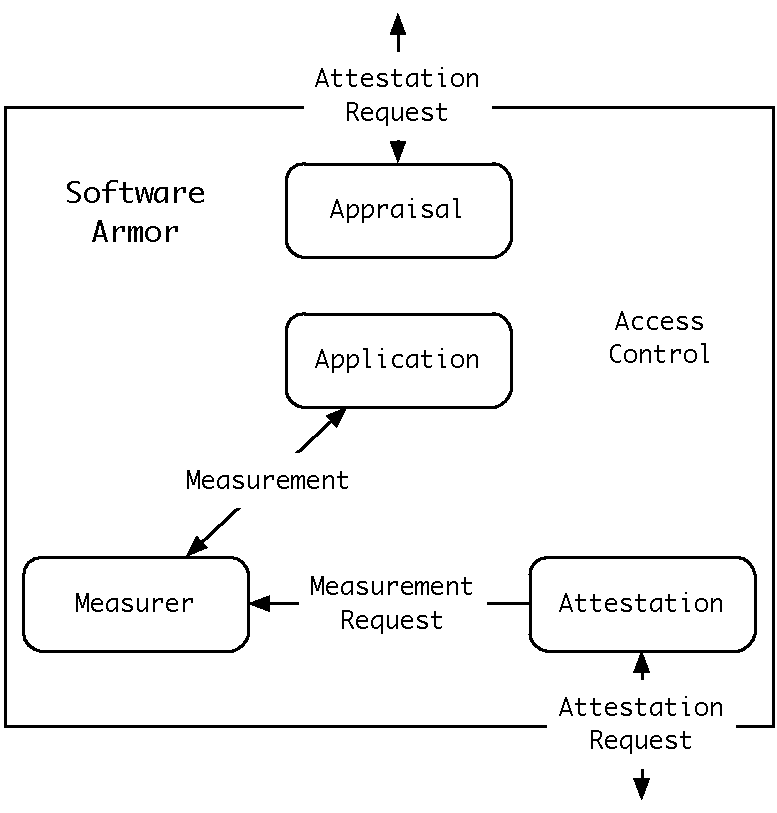
\includegraphics[width=0.95\textwidth]{figures/architecture.pdf}
  \caption{\textsc{ArmoredSoftware} component architecture showing
    major components of the remote attestation process.}
  \label{fig:architecture}
\end{marginfigure}

Figure~\ref{fig:architecture} depicts interactions among major
architectural components of a protected \textsc{ArmoredSoftware}
application.  The \emph{Application} is the running program to be
protected by the infrastructure.  It need not be modified or aware of
the other armor components unless desired by the user.  An
\emph{Appraiser} initiates trust assessment by requesting information
from the operational environment, other \textsc{ArmoredSoftware}
applications and traditional cloud applications to assess the
operational environment.  The Appraiser specifies what information it
needs without specifying how that information should be gathered.  The
\emph{Attestation Manager} receives a request from an Appraiser and
selects an attestation protocol to fulfill the Appraiser's request.
It then executes that protocol to gather evidence by invoking
measurers along with cryptographic assurance of integrity and
confidentiality.  It also provides evidence of correct protocol
execution and correct Measurer interaction.  The \emph{Measurer}
performs specific measurement operations on the running application
and returns evidence describing application operation. Measurers are
specialized for their associated software application and may range
from gathering simple values to observing operational state over time.
Using evidence gathered by the Measurer and returned by the
Attestation Manager, the Appraiser directs response to appraisal.
Such responses may include migration, reporting, or shutdown.
\emph{Access control} governs access to all critical resources in the
protected application to assure secrets are preserved and enforce
information flow restrictions.

\newthought{The \textsc{ArmoredSoftware} approach has} three
significant advantages: (i) flexibility; (ii) simplicity; and (iii)
usability.  The use of protocols to perform attestation allows
operations ranging from simple operational checks to complex
interactions among many \textsc{ArmoredSoftware} components.  The use
of application specific Measurers allows specialization to the
component resulting in simpler, more effective evidence gathering.
Finally, \textsc{ArmoredSoftware} does not require modification of
cloud applications.  While users will write applications to take
advantage of \textsc{ArmoredSoftware} capabilities, existing
applications can be reused without modification.

% Figure~\ref{fig:architecture} graphically represents the interaction among
% protected components while Figure~\ref{fig:system} shows the
% sequencing of interactions during appraisal.  A component's appraisal
% module will request information from a second component's attestation
% module.  The attestation model will select an attestation protocol
% that instructs the measurer what information to gather and in what
% sequence.  The measurer executes that protocol that in turn gathers
% information from the running process, accesses the module's virtual
% TPM (vTPM) and makes appraisal requests of other
% \textsc{ArmoredSoftware} instances.  The attestation module assembles
% measurement results into a evidence package that is returned to the
% requesting appraiser with cryptographic assurances of integrity and
% confidentiality as required.  Upon receiving the package, the
% appraiser assesses cryptographic signatures and encryption to
% determine the trustworthiness of the measurements, then assesses
% measurements to determine the trustworthiness of the component being
% appraised.

% \begin{figure}[hbtp]
%   \centering
%   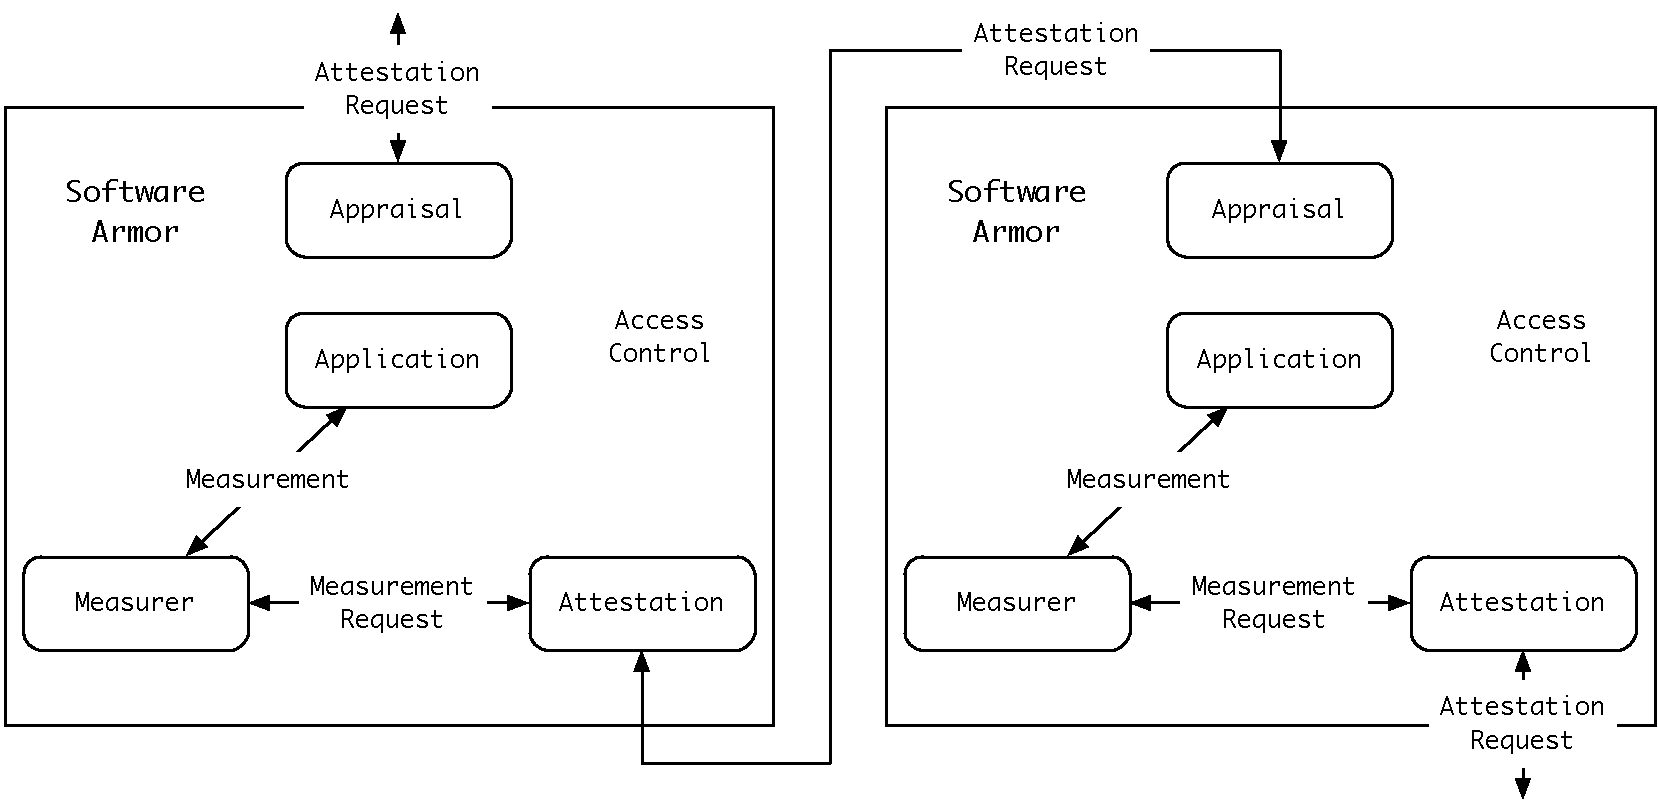
\includegraphics[width=0.85\textwidth]{figures/system.pdf}
%   \caption{Typical interaction among armored components with an
%     appraiser interacting with an attestation agent to gather
%     information.}
%   \label{fig:system}
% \end{figure}

\bibliography{onePager}

\end{document}
